\section{Problems}
%% TEMPLATE STUFF - WORK BELOW THIS BLOCK
%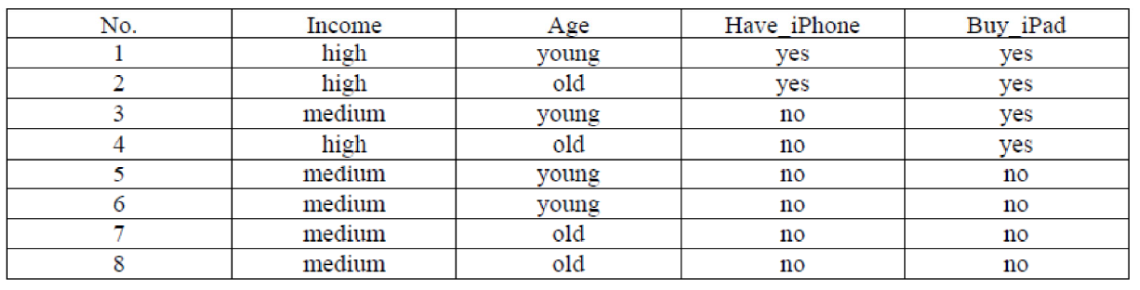
\includegraphics[width=1\textwidth]{media/hw5_q1.png}
%\begin{align}
%    P(I=m | iPad = y) &= \frac{1}{4} \label{eq:q1_1} \nonumber \\
%    P(I=m | iPad = n) &= \frac{4}{4} = 1
%\end{align}

\subsection{Question One}
The method called “bagging” was not discussed in class lecture. “Bagging” is a short name of Bootstrap Aggregating. We would like you to self-study this concept via ChatGPT or any other online materials you trust. Bagging is not a model evaluation method but a model training method.

\textbf{(a) Please describe the procedure of Bagging.}

Bagging, short for Bootstrap Aggregating, is an ensemble learning technique designed to improve the stability and accuracy of machine learning algorithms. The procedure of bagging can be described in the following steps:

\begin{itemize}
    \item \textbf{Bootstrap Sampling}: Create multiple subsets of the original training dataset by randomly sampling with replacement. Each subset, known as a bootstrap sample, may contain duplicate instances and will typically be of the same size as the original dataset.

    \item \textbf{Train Base Learners}: For each bootstrap sample, train a separate base learner (e.g., decision tree, neural network). Each model is trained independently, and the randomness introduced by bootstrap sampling ensures that the models capture different patterns in the data.

    \item \textbf{Aggregate Predictions}: Once all base learners are trained, aggregate their predictions to make a final prediction. For classification tasks, the most common aggregation method is majority voting, where the class predicted by the majority of the models is chosen. For regression tasks, the predictions are typically averaged.

    \item \textbf{Final Model Output}: The output of the bagging procedure is a single ensemble model that combines the strengths of all the individual base learners, often leading to improved performance and reduced variance compared to any single model.

    \item \textbf{Evaluation and Tuning}: After constructing the bagging ensemble, evaluate its performance on a validation dataset. Hyperparameters, such as the number of base learners or the type of base learner, can be tuned to optimize performance further.
\end{itemize}

\textbf{(b) Why Bagging generally reduce model variance?}

Bagging (Bootstrap Aggregating) generally reduces model variance due to the following reasons:

\begin{itemize}
    \item \textbf{Independence of Base Learners}: By training multiple models on different bootstrap samples of the data, bagging introduces diversity among the base learners. Each model captures different aspects of the data, which helps to smooth out the predictions when aggregated.

    \item \textbf{Averaging Effect}: In regression tasks, the predictions from the individual models are averaged, while in classification tasks, majority voting is used. This aggregation process tends to cancel out the errors made by individual models. If one model makes a high variance error due to a particular subset of data, other models are less likely to make the same mistake, leading to a more stable overall prediction.

    \item \textbf{Reduction of Overfitting}: Models with high variance often overfit the training data, capturing noise and specific patterns that do not generalize well to new data. Bagging mitigates this effect by combining the outputs of multiple models, each trained on slightly different data, which can lead to a more generalized model that performs better on unseen data.

    \item \textbf{Error Reduction through Diversity}: When base learners are trained on different samples, they are likely to make different errors. The aggregation of these diverse predictions helps to reduce the overall error, resulting in lower variance in the ensemble model compared to individual models.

    \item \textbf{Robustness to Outliers}: Bagging is more robust to outliers since the influence of any single data point is diminished across the ensemble. As each model sees a different subset of the data, the impact of outliers on the final prediction is reduced.
\end{itemize}

\subsection{Support Vector Machine}
\textbf{(a) [10 pts] The following is the primal formulation of L2 SVM (with the squared slack variables), which is a variant of the standard SVM that we discussed in our lecture. }

\begin{align}
    \min_{w, b, \xi} \quad & \frac{1}{2} \mathbf{w}^T \mathbf{w} + \frac{C}{2} \sum_{i=1}^{N} \xi_i^2 \label{eq:svm_objective} \\
    \text{s.t.} \quad & y_i (\mathbf{w}^T \mathbf{x}_i + b) \geq 1 - \xi_i, \quad i \in \{1, \ldots, N\}, \label{eq:svm_constraint1} \\
    & \xi_i \geq 0, \quad i \in \{1, \ldots, N\}. \label{eq:svm_constraint2}
\end{align}




If we remove the last constraints \((\xi_i \geq 0)\), we might get a simpler optimization problem:

\begin{align}
    \min_{w, b, \xi} \quad & \frac{1}{2} \mathbf{w}^T \mathbf{w} + \frac{C}{2} \sum_{i=1}^{N} \xi_i^2 \label{eq:svm_objective} \\
    \text{s.t.} \quad & y_i (\mathbf{w}^T \mathbf{x}_i + b) \geq 1 - \xi_i, \quad i \in \{1, \ldots, N\}. \label{eq:svm_constraint}
\end{align}


\textbf{Please provide the Lagrangian of the above simplified formulation.}

The Lagrangian for the simplified primal formulation of L2 SVM, where the last constraint \(\xi_i \geq 0\) is removed, can be formulated as follows:

The simplified optimization problem is:

\[
\min_{w, b, \xi} \quad \frac{1}{2} \mathbf{w}^T \mathbf{w} + \frac{C}{2} \sum_{i=1}^{N} \xi_i^2
\]

subject to the constraints:

\[
y_i (\mathbf{w}^T \mathbf{x}_i + b) \geq 1 - \xi_i, \quad \forall i \in \{1, \ldots, N\}
\]

The Lagrangian \(\mathcal{L}\) is formed by incorporating the constraints with Lagrange multipliers \(\alpha_i\):

\[
\mathcal{L}(w, b, \xi, \alpha) = \frac{1}{2} \mathbf{w}^T \mathbf{w} + \frac{C}{2} \sum_{i=1}^{N} \xi_i^2 - \sum_{i=1}^{N} \alpha_i \left( y_i (\mathbf{w}^T \mathbf{x}_i + b) - (1 - \xi_i) \right)
\]

where:
- \(\alpha_i \geq 0\) are the Lagrange multipliers corresponding to each constraint.

The Lagrangian combines the original objective function and the penalty for violating the constraints, which will be optimized along with the primal variables \(w\), \(b\), and \(\xi\).


\textbf{(b) [15 pts] Please find the partial derivative of the Lagrangian in (a) with respect to $w$, $b$, and $\xi_i$.
}

The Lagrangian from part (a) is given by:

\[
\mathcal{L}(\mathbf{w}, b, \xi, \alpha) = \frac{1}{2} \mathbf{w}^T \mathbf{w} + \frac{C}{2} \sum_{i=1}^{N} \xi_i^2 - \sum_{i=1}^{N} \alpha_i \left( y_i (\mathbf{w}^T \mathbf{x}_i + b) - (1 - \xi_i) \right)
\]

We need to compute the partial derivatives with respect to \( \mathbf{w} \), \( b \), and \( \xi_i \):

1. **Partial Derivative with respect to \( \mathbf{w} \)**:

\[
\frac{\partial \mathcal{L}}{\partial \mathbf{w}} = \mathbf{w} - \sum_{i=1}^{N} \alpha_i y_i \mathbf{x}_i
\]

2. **Partial Derivative with respect to \( b \)**:

\[
\frac{\partial \mathcal{L}}{\partial b} = -\sum_{i=1}^{N} \alpha_i y_i
\]

3. **Partial Derivative with respect to \( \xi_i \)**:

\[
\frac{\partial \mathcal{L}}{\partial \xi_i} = C \xi_i - \alpha_i
\]

These partial derivatives are essential for setting up the conditions for optimality in the optimization problem of the L2 SVM formulation.


\subsection{Cluster Analysis}

\textbf{[25 pts]} Consider the following set of one-dimensional data points: \{0.1, 0.25, 0.45, 0.55, 0.8, 0.9\}. All the points are located in the range between [0, 1].

\textbf{(a) [15 pts]} Suppose we apply K-Means clustering to obtain three clusters, A, B, and C. If the initial centroids are located at \{0, 0.4, 1\}, respectively, show the cluster assignments and locations of the updated centroids after the first three iterations by filling out the following table. (Hint: although you can directly calculate all distances, if you draw a real axis and put down the points, it might be easier to see the cluster assignment.)

\begin{table}[h]
\centering
\begin{tabular}{|c|c|c|c|c|c|c|}
\hline
\text{Iter} & \text{Cluster assignment of data points} & \text{Centroid Location} \\
\hline
0 & 0.10, 0.25 & A \\
  & 0.45, 0.55 & B \\
  & 0.80, 0.90 & C \\
\hline
1 & 0.10, 0.25 & A (0.175) \\
  & 0.45, 0.55 & B (0.5) \\
  & 0.80, 0.90 & C (0.95) \\
\hline
2 & 0.10, 0.25 & A (0.175) \\
  & 0.45, 0.55, 0.80 & B (0.55) \\
  & 0.90 & C (0.90) \\
\hline
3 & 0.10, 0.25 & A (0.175) \\
  & 0.45, 0.55, 0.80 & B (0.55) \\
  & 0.90 & C (0.90) \\
\hline
\end{tabular}
\caption{K-Means clustering results after three iterations.}
\end{table}

\textbf{(b) [5 pts]} Find the sum-of-squared errors (SSE) of the clustering after the third iteration.

To calculate the SSE, we need to compute the squared distances of each data point from its respective cluster centroid.

\[
\text{SSE} = \sum_{i=1}^{k} \sum_{x_j \in C_i} (x_j - \mu_i)^2
\]

Where:
- \( \mu_i \) is the centroid of cluster \( C_i \).
- \( x_j \) is a data point in cluster \( C_i \).

For the clusters after the third iteration:

- **Cluster A**: Centroid = 0.175
    - Points: 0.1, 0.25
    - \( \text{SSE}_A = (0.1 - 0.175)^2 + (0.25 - 0.175)^2 = 0.005625 + 0.005625 = 0.01125 \)

- **Cluster B**: Centroid = 0.55
    - Points: 0.45, 0.55, 0.8
    - \( \text{SSE}_B = (0.45 - 0.55)^2 + (0.55 - 0.55)^2 + (0.8 - 0.55)^2 = 0.010000 + 0 + 0.062500 = 0.072500 \)

- **Cluster C**: Centroid = 0.90
    - Points: 0.90
    - \( \text{SSE}_C = (0.9 - 0.90)^2 = 0 \)

Thus, the total SSE is:

\[
\text{SSE} = \text{SSE}_A + \text{SSE}_B + \text{SSE}_C = 0.01125 + 0.0725 + 0 = 0.08375
\]

\textbf{(c) [5 pts]} For the dataset given in part (1), is it possible to obtain empty clusters? Why?

Yes, it is possible to obtain empty clusters in K-Means clustering, particularly when the initial centroids are poorly chosen. 

In the context of the dataset \{0.1, 0.25, 0.45, 0.55, 0.8, 0.9\} and the initial centroids \{0, 0.4, 1\}, the following scenarios can lead to empty clusters:

1. **Poor Initialization**: If the initial centroids are chosen such that no data points are close enough to a particular centroid, that cluster will remain empty throughout the iterations. For instance, if the centroid at 1 does not have any data points near it, it may end up being an empty cluster.

2. **Distance-based Assignments**: During the assignment step of K-Means, each data point is assigned to the nearest centroid. If the distances are such that all points are closer to the other centroids (e.g., points being closer to centroid 0 or 0.4), then the centroid at 1 will have no points assigned to it, leading to an empty cluster.

Thus, the occurrence of empty clusters is primarily influenced by the selection of initial centroids and the distribution of the data points.


